\documentclass[
  fontsize=10pt,
  %oneside,
  %open=any,
  %chapterprefix=true,
  numbers=noenddot,
  %draft,
]{../kaobook}

% Load common packages and commands
\usepackage{../packages}
\usepackage{../commands}
\usepackage{../style}

% Load packages for testing
\usepackage{blindtext}
%\usepackage{showframe}
%\usepackage{showlabels}

% Add bibfile
\addbibresource{main.bib}

% Set path for images
\graphicspath{{images/}{../images/}}

% Index
\makeindex[columns=3, title=Alphabetical Index, intoc]

% Glossary
\makeglossaries

\begin{document}

% General structure of a book:
% 	\frontmatter
% 	Cover
% 	Half-title (r)
% 	Frontispiece (v)
% 	Title (r)
%	Information (copyright, ISBN, etc.) (v)
%	Dedication (r)
%	Notation and other conventions used (v)
%	Table of contents (r)
%	List of figures (r)
%	Preface (r)
%
%	\mainmatter
%	Chapters (1, 2, ..., n)
%
%	\appendix
%	Appendices (A, B, ..., Z)
%
%	\backmatter
%	Bibliography (r)
%	Glossary (r)
%	Index (r)
%	Empty
%
%	Cover

\titlehead{The \texttt{kaobook} class}
\subject{Use this document as a template}
\title[Example and Documentation of the \texttt{kaobook} class]{Example 
	and Documentation \\ of the \texttt{kaobook} class}
\subtitle{Customise this page according to your needs}
\author[Federico Marotta]{Federico Marotta \thanks{A \LaTeX\ lover}}
\date{\today}
\publishers{an Awesome Publisher}

\frontmatter

%\includepdf{pages/cover-front.pdf}

% Half-title

\makeatletter
\extratitle{
	% In the title page, the title is vspaced by 9.5\baselineskip
	\vspace*{9\baselineskip}
	\vspace*{\parskip}
	\begin{center}
		% In the title page, \huge is set after the komafont for title
		\usekomafont{title}\huge\@title
	\end{center}
}
\makeatother


% Frontispiece (verso of the half-title)

\frontispiece{}


% Copyright page
\makeatletter
\uppertitleback{\@titlehead}

\lowertitleback{
\textbf{Disclaimer}\\
You can edit this page to suit your needs. For instance, here we have a 
no copyright statement, a colophon and some other information. This page 
is based on the corresponding page of Ken Arroyo Ohori's thesis, with 
minimal changes.

\textbf{No copyright}\\
\cczero\ This thesis is released into the public domain using the CC0 code.
To the extent possible under law, I waive all copyright and related or neighbouring rights to this work.

To view a copy of the CC0 code, visit: \\
\url{http://creativecommons.org/publicdomain/zero/1.0/}

\textbf{Colophon} \\
This document was typeset with the help of 
\href{https://sourceforge.net/projects/koma-script/}{\KOMAScript} and
\href{ttps://www.latex-project.org/}{\LaTeX} using the 
\href{https://github.com/fmarotta/kaobook/}{kaobook} class.

The source code of this thesis is available at: \\
\url{https://myurl.com}

\textbf{Publisher} \\
First printed in Jan 2019 by \@publishers
}
\makeatother


% Dedication page

\dedication{
	The harmony of the world is made manifest in Form and Number, and 
	the heart and soul and all the poetry of Natural Philosophy are 
	embodied in the concept of mathematical beauty.\\
	\flushright -- D'Arcy Wentworth Thompson
}


\begin{titlepage}
\vbox{ }

\vbox{ }

\begin{center}
% Upper part of the page

\includegraphics[width=0.25\textwidth]{./sections/img/overleaf-logo}\\[1cm]
\textsc{\LARGE Overleaf Team}\\[1.5cm]
\textsc{\Large Testing Example}\\[0.5cm]

\vbox{ }
% Title
\HRule \\[0.4cm]
{ \huge \bfseries Creating a large project}\\[0.4cm]
\HRule \\[1.5cm]
% Author and supervisor
\begin{minipage}{0.4\textwidth}
\begin{flushleft} \large
\emph{Author:}\\
Gubert Farnsworth
\end{flushleft}
\end{minipage}
\begin{minipage}{0.4\textwidth}
\begin{flushright} \large
\emph{Special colaborator:} \\
John Doe
\end{flushright}
\end{minipage}
\vfill
% Bottom of the page
{\large July, 2021}
\end{center}
\end{titlepage}


%% Greek alphabet with pronunciation (borrowed from
% https://gitlab.com/jim.hefferon/linear-algebra)
\thispagestyle{empty}

\begin{center}
  \textbf{Greek letters with pronounciation}
    \\[1.5ex]
  \newcommand{\pronounced}[1]{\hspace*{.2em}\small\textit{#1}}
  \begin{tabular}{cl@{\hspace*{3em}}cl}
    character &\multicolumn{1}{c}{\makebox[-3.5em][r]{name}}       
    &character  &\multicolumn{1}{c}{\makebox[-3.5em][r]{name}}  \\ 
    \hline
     \makebox[1em][l]{\( \alpha  \)} &alpha \pronounced{AL-fuh}  
       &\makebox[1em][l]{\( \nu     \)}  &nu  \pronounced{NEW}       \\
     \makebox[1em][l]{\( \beta   \)} &beta  \pronounced{BAY-tuh}     
       &\makebox[1em][l]{\( \xi  \), \( \Xi \)}  &xi   \pronounced{KSIGH}    \\ 
     \makebox[1em][l]{\( \gamma  \), \( \Gamma \)} &gamma  \pronounced{GAM-muh}
       &\makebox[1em][l]{\( o \)} &omicron  \pronounced{OM-uh-CRON}  \\
     \makebox[1em][l]{\( \delta  \), \( \Delta \)} &delta  \pronounced{DEL-tuh} 
       &\makebox[1em][l]{\( \pi \), \( \Pi \)} &pi  \pronounced{PIE}     \\
     \makebox[1em][l]{\( \epsilon\)} &epsilon  \pronounced{EP-suh-lon}   
       &\makebox[1em][l]{\( \rho \)} &rho  \pronounced{ROW}    \\
     \makebox[1em][l]{\( \zeta   \)} &zeta   \pronounced{ZAY-tuh}    
       &\makebox[1em][l]{\( \sigma  \), \( \Sigma \)} &sigma  \pronounced{SIG-muh}  \\
     \makebox[1em][l]{\( \eta  \)} &eta  \pronounced{AY-tuh}      
       &\makebox[1em][l]{\( \tau \)} &tau  \pronounced{TOW (as in cow)}    \\
     \makebox[1em][l]{\( \theta \), \( \Theta \)} &theta  \pronounced{THAY-tuh}    
       &\makebox[1em][l]{\( \upsilon\), \( \Upsilon \)} &upsilon  \pronounced{OOP-suh-LON}  \\
     \makebox[1em][l]{\( \iota \)} &iota \pronounced{eye-OH-tuh}   
       &\makebox[1em][l]{\( \phi \), \( \Phi \)} &phi  \pronounced{FEE, or FI (as in hi)}    \\
     \makebox[1em][l]{\( \kappa  \)} &kappa  \pronounced{KAP-uh}  
       &\makebox[1em][l]{\( \chi \)}  &chi  \pronounced{KI (as in hi)}    \\
     \makebox[1em][l]{\( \lambda \), \( \Lambda \)} &lambda  \pronounced{LAM-duh}  
       &\makebox[1em][l]{\( \psi    \), \( \Psi \)}  &psi \pronounced{SIGH, or PSIGH}    \\
     \makebox[1em][l]{\( \mu  \)}  &mu  \pronounced{MEW}     
       &\makebox[1em][l]{\( \omega  \), \( \Omega \)} &omega  \pronounced{oh-MAY-guh}  
  \end{tabular}   \\[1.5ex]
  Capitals shown are the ones that differ from Roman capitals.
\end{center}


%%%%%%%%%%%%%%%%%%%%%%preface.tex%%%%%%%%%%%%%%%%%%%%%%%%%%%%%%%%%%%%%%%%%
% sample preface
%
% Use this file as a template for your own input.
%
%%%%%%%%%%%%%%%%%%%%%%%% Springer %%%%%%%%%%%%%%%%%%%%%%%%%%

\preface

%% Please write your preface here
Use the template \emph{preface.tex} together with the Springer document class SVMono (monograph-type books) or SVMult (edited books) to style your preface in the Springer layout.

A preface\index{preface} is a book's preliminary statement, usually written by the \textit{author or editor} of a work, which states its origin, scope, purpose, plan, and intended audience, and which sometimes includes afterthoughts and acknowledgments of assistance. 

When written by a person other than the author, it is called a foreword. The preface or foreword is distinct from the introduction, which deals with the subject of the work.

Customarily \textit{acknowledgments} are included as last part of the preface.
 

\vspace{\baselineskip}
\begin{flushright}\noindent
Place(s),\hfill {\it Firstname  Surname}\\
month year\hfill {\it Firstname  Surname}\\
\end{flushright}




\begingroup
%\etocstandarddisplaystyle
%\etocstandardlines
%\etocmulticolstyle[2]{\chapter*{Contents}}
\tableofcontents
\listoffigures
\listoftables
\endgroup


\mainmatter

\renewcommand*{\chapterformat}
{
  \enskip\mbox{\scalebox{4}{\thechapter\autodot}}
}
\renewcommand\chapterlinesformat[3]
{
  \vspace*{-1cm}%
  \parbox[b]{\textwidth}{\hrulefill#2}\par%
  #3%\par\bigskip
  \parbox[b]{\textwidth+\marginparsep+\marginparwidth}{\hrulefill}%
  %\hrule
}
\setchapterpreamble[u]{\margintoc}
\chapter{Introduction}

\section{The main ideas}

Many modern printed textbooks have adopted a layout with prominent 
margins where small figures, tables, remarks and just about everything 
else can be displayed. Arguably, this layout helps to organise the 
discussion by separating the main text from the ancillary material, 
which at the same time is very close to the point in the text where it 
is referenced.

This text does not aim to be an apology of wide margins, for there are 
many better suited authors for this task; the purpose of all these words 
is just to fill the space so that the reader can see how a book written 
with the kaobook class looks like. Meanwhile, I shall also try to 
illustrate the features of the class.

The main ideas behind kaobook come from this 
\href{https://3d.bk.tudelft.nl/ken/en/2016/04/17/a-1.5-column-layout-in-latex.html}{blog 
	post}, and actually the name of the class is dedicated to the author 
of the post, Ken Arroyo Ohori, which has kindly allowed me to create a 
class based on his thesis. Therefore, if you want to know more reasons 
to prefer a 1.5-column layout for your books, you can read his blog 
post.

\section{What this class does}
\labsec{does}

The kaobook class focuses more about the document structure than about 
the style. Indeed, it is a well-known \LaTeX\xspace printiple that 
structure and style should be separated as much as possible (see also 
\refsec{doesnot}). This means that this class will only provide 
commands, environments and in general, the opportunity to do things, 
which the user may or may not exploit. Actually, some stylistic matters 
are embedded in the class, but the user is able to customise them with 
ease.

The main features are the following:

\begin{description}
	\item[Page Headings] They span the margins and, in twoside mode, 
		display alternatively the chapter and the section name.
	\item[Matters] The commands \verb|\frontmatter|, \verb|\mainmatter| 
		and \verb|\backmatter| have been redefined in order to have 
		automatically wide margins in the main matter, and narrow 
		margins in the front and back matters.
	\item[Margin text] We provide commands \verb|\sidenote| and 
		\verb|\marginnote| to put text in the margins\sidenote{Sidenotes 
			(like this!) are numbered while marginnotes are not}.
	\item[Margin figs/tabs] A couple of useful environments is 
		\verb|marginfigure| and \verb|margintable|, which, not 
		surprisingly, allow you to put figures and tables in the margins 
		(cfr. \reffig{marginmonalisa}).
		\begin{marginfigure}[*-3]
			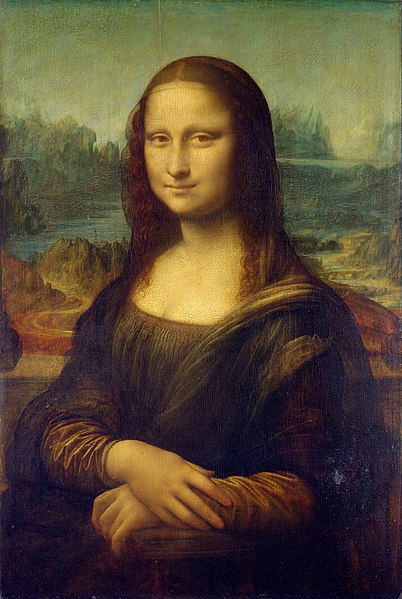
\includegraphics{monalisa}
			\caption[The Mona Lisa]{The Mona Lisa.\\
				\url{https://commons.wikimedia.org/wiki/File:Mona_Lisa,_by_Leonardo_da_Vinci,_from_C2RMF_retouched.jpg}}
			\labfig{marginmonalisa}
		\end{marginfigure}
	\item[Margin toc] Finally, since we have wide margins, why don't add 
		a little table of contents in them? See \verb|\margintoc| for 
		that.
	\item[Hyperref] \verb|hyperref| is loaded and by default we try to 
		add bookmarks in a sensible way; in particular, the bookmarks 
		levels are automatically reset at \verb|\appendix| and 
		\verb|\backmatter|.
\end{description}

\section{What this class does not}
\labsec{doesnot}

As anticipated, the styling is left to the user. Indeed, every book may 
have sidenotes, margin figures and so on, but each book will have its 
own fonts, toc style and so on. For this reason, we only provide 
sensible defaults. The github repository is organised as follows.

\begin{description}
	\item[kaobook.cls] The class file, which contains the definitions of 
		the commands and the environments and loads the required 
		packages.
	\item[packages.sty] Loads other packages to improve the experience 
		of the user (for instance, \verb|ams*| packages are loaded here 
		as they are not required in every book).
	\item[commands.sty] Complements to the packages, \eg the 
		specifications of the \verb|theorem| environments.
	\item[style.sty] Page layout, formatting of the titles\ldots
\end{description}

Moreover, there is a folder containing this very book as an example.


\widepage
\setpartpreamble{
  \begin{center}
  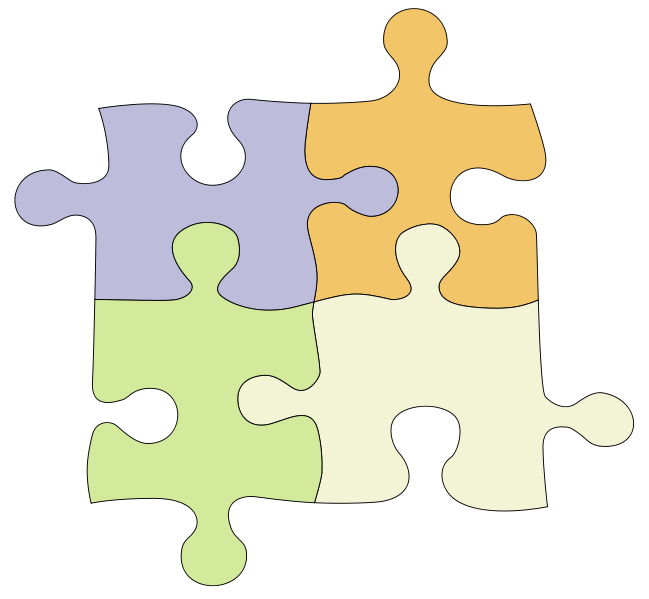
\includegraphics[width=0.8\linewidth]{images/partpre}
  \captionof{figure}{\url{https://commons.wikimedia.org/wiki/File:Puzzle-4.svg}}
  \end{center}
}
\part{Class Options, Commands and Environments}
\marginpage

\renewcommand*{\chapterformat}
{
  \enskip\mbox{\scalebox{3.5}{\framebox{\thechapter\autodot}}}
}
\renewcommand\chapterlinesformat[3]
{
  \parbox[b]{\textwidth+\marginparsep+\marginparwidth}{
	\parbox[b]{\textwidth}{#3}%
	\parbox[b]{\marginparsep}{\hfill}%
	\parbox[b]{\marginparwidth}{#2}%
  }
  %\hrule
}
\setchapterpreamble[u]{\margintoc[*-3]}
\chapter{Class Options}

In this chapter I will describe the most common options used, both the 
ones inherited from scrbook and the kao-specific ones.

\section{KOMA options}

The class is based on the scrbook, therefore it understands all of the 
options you would normally pass to that class. By default, the font size 
is 9pt and the paragraphs are separated by space, not marked by 
indentation. The default value for parskip is half.

The toc has an entry for everything: listoffigures, listoftables, 
indices, and bibliographies. There are also entries for the 
tableofcontents itself (through the \verb|\setuptoc{toc}{totoc}| 
command). If you want entries for the glossaries as well, you can set 
the \verb|toc| option of the package \verb|glossaries|.

\section{kao options}

In the future I plan to add more options to set the paragraph formatting 
(justified vs ragged) and the position of the margins (inner vs outer in 
twoside mode, left vs right in oneside mode)\sidenote{As of now, 
	paragraphs are justified, formatted with \texttt{singlespacing} 
	(from package \texttt{setspace}) and \texttt{frenchspacing}.}. 

\section{Other things worth knowing}

By default, dispositions are numbered up to the section thanks to the 
command \verb|\setcounter{secnumdepth}{1}|. We also altered slightly the 
entries of the parts in the table of contents so as to include "Part". 
The table of contents can be modified through the package \verb|etoc|, 
which is loaded because it is needed for the margintocs.

\marginnote[1.5\parskip]{We also load \texttt{xcolor}.}

The packages \verb|inputenc|, \verb|hyphenat|, \verb|microtype| are 
already loaded, but you have to load babel or polyglossia and csquotes, 
if you wish.

\section{Document Structure}

We provide optional arguments to the \verb|\title| and \verb|\author| 
commands so that you can insert short, plain text versions of this 
fields, which can be used, typically in the half-title or somewhere else 
in the frontmatter, through the commands \verb|\@plaintitle| and 
\verb|\@plainauthor|, respectively. The pdftitle and pdfauthor are set 
through hyperref to the plain values if present, otherwise to the normal 
values.

The frontmatter uses a layout without margins and a plain page style 
(\ie no headings). In the mainmatter the margins are wide, the page 
numbers are arabic (while in the frontmatter there are roman numbers) 
and the headings are fancy. In the appendix we use 
\verb|\bookmarksetup{startatroot}| so that the bookmarks to the chapters 
are on their own; without this, they would be under the previous part. 
In the backmatter the margins shrink again and we reset again the 
bookmarks root.

\renewcommand*{\chapterformat}
{
  \enskip\mbox{\scalebox{4}{\thechapter\autodot}}
}
\renewcommand\chapterlinesformat[3]
{
  \parbox[b]{\textwidth+\marginparsep+\marginparwidth}{\hrulefill#2}\par%
  #3%
  %\parbox[b]{\textwidth+\marginparsep+\marginparwidth}{\hrulefill}%
}
\setchapterpreamble[u]{\margintoc}
\chapter{Sidenotes and Marginnotes}

\section{Sidenotes}

To insert a sidenote, just enter the command \verb|\sidenote{Text of the note}|. You can specify a mark\sidenote[O]{This sidenote has a 
	special mark} with \verb|\sidenote[mark]{Text}|, or you can specify 
an offset and a mark with \verb|\sidenote[offset][mark]{Text}|, in which 
case the mark can be empty. If you want to know more, read the 
documentation of the \verb|snotez| package.

Sidenotes are handled through the \verb|snotez| package, which relies on 
the \verb|marginnote| package. The sidenote counter is never reset, but 
if you want you can reset it at every chapter.

\section{Marginnotes}

\marginnote{\blindtext}

\subsection{Usage}

This command is similar to the previous one: you can use it like 
\verb|\marginnote[offset]{Text}|, where the offset argument can be left 
out.

\subsection{Details}

We load the packages \verb|marginnote|, \verb|marginfix| and 
\verb|placeins|. Since \verb|snotez| uses \verb|marginnote|, what we say 
for marginnotes is also valid for sidenotes. The style of marginnotes 
and captions is the same, and the notes are shifted slightly upwards 
(\verb|\renewcommand{\marginnotevadjust}{-11pt}|) in order to allineate 
them to the bottom of the line of text where the marginnote is issued.

\marginnote[*-1.5]{The offset option can be either a length or a 
	multiple of \texttt{baselineskip}, \eg 
	\texttt{\\marginnote[*-3]{Text}}.}

\section{Footnotes}

Footnotes force the reader to constantly move from one area of the page 
to the other. Arguably marginnotes solve this issue, so you should not 
use footnotes. Nevertheless, for completeness, we provide the standard 
command \verb|\footnote|, just in case you want to put a footnote once 
in a while\footnote{And this is how they look like.}.

\section{Margintoc}

Since we are talking about margins, we introduce here the 
\verb|\margintoc| command, which accepts a parameter for the vertical 
offset, like so: \verb|\margintoc[offset]|. It can be used in any point 
of the document, but we think it makes sense to use it at the beginning 
of chapters or parts. We like to put it in the chapter preamble, with 
this code:

\begin{verbatim}
	\setchapterpreamble[u]{\margintoc}
	\chapter{Sidenotes and Marginnotes}
\end{verbatim}

\setchapterpreamble[o]{
	\begingroup
	\vspace*{-2.60cm}\hspace*{-2.25cm}
	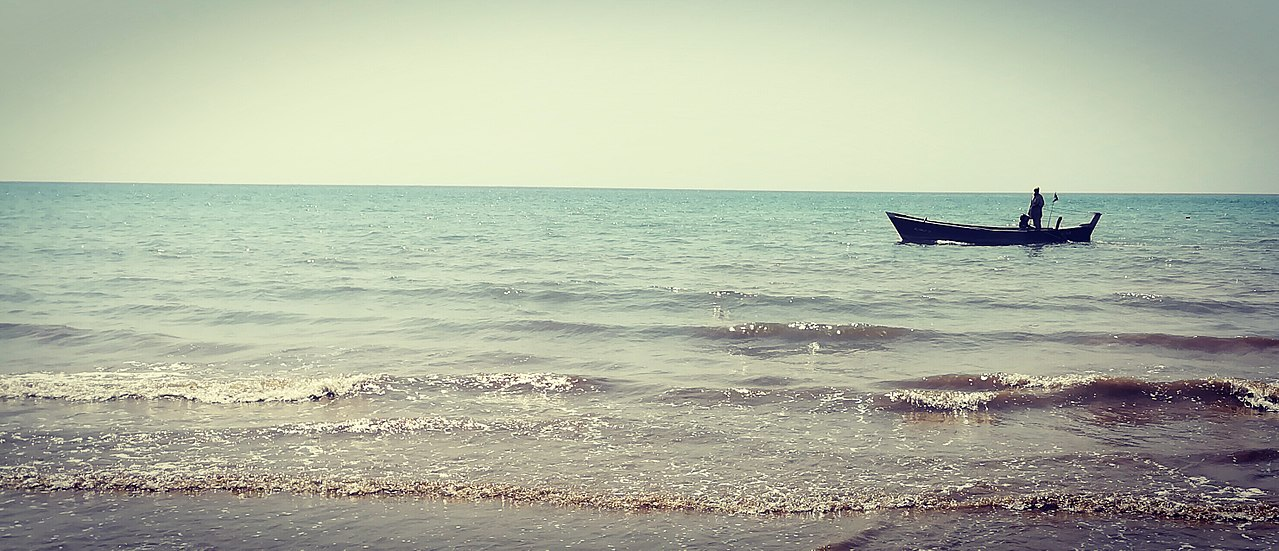
\includegraphics[width=\paperwidth,height=8cm,keepaspectratio=false]{images/seaside}
	\vspace{-1.0cm}
	\addtokomafont{captionlabel}{\bfseries}
	\captionsetup{
		type=figure,
		format=marginemph, 
		width=\textwidth+\marginparsep+\marginparwidth,
		%indention=2cm,
		parindent=0.7cm,
	}
	\caption[The seaside]{By Bushra Feroz - Own work, CC BY-SA 4.0, 
		https://commons.wikimedia.org/w/index.php?curid=68724647}
	\endgroup
}
% beforeskip=-(figure_height-top_margin)
\RedeclareSectionCommand[beforeskip=-5.3cm]{chapter}
\setchapterpreamble[u]{\margintoc[*-4.5]}

\makeatletter
\renewcommand{\chapterlinesformat}[3]{%
  \@hangfrom{#2}{#3}%
}
\makeatother
\renewcommand*{\chapterformat}{%
  \mbox{\chapappifchapterprefix{\nobreakspace}\thechapter
	\autodot\IfUsePrefixLine{}{\enskip}}}

\chapter{Figures and Tables}
\RedeclareSectionCommand[beforeskip=0cm]{chapter}

\section{Normal figures and tables}

Normal figures and tables can be inserted just like in any standard 
\LaTeX\xspace document. The captions will be positioned in the margins 
thanks to the \verb|floatrow| package. The space between the figure and 
the text can be specified with the following commands:

\begin{verbatim}
	\renewcommand\FBaskip{4pt}
	\renewcommand\FBbskip{4pt}
\end{verbatim}

Here is a picture of Mona Lisa (\reffig{normalmonalisa}), as an example. 
The captions are formatted as the marginnotes; to change the options you 
can use \verb|\captsetup| from the \verb|caption| package.

\begin{figure}[h]
	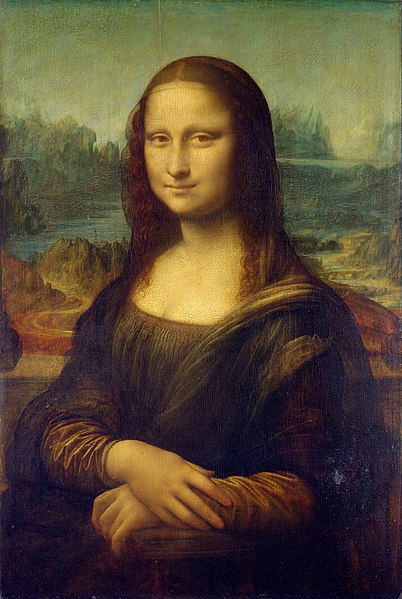
\includegraphics[width=0.4\textwidth]{monalisa}
	\caption[Mona Lisa, again]{It's Mona Lisa again. \blindtext}
	\labfig{normalmonalisa}
\end{figure}

I don't have much to say, so I will just insert some blind text. 
\blindtext

\begin{table}
\begin{tabular}{ |c|c|c|c| } 
\hline
col1 & col2 & col3 \\
\hline
\multirow{3}{4em}{Multiple row} & cell2 & cell3 \\ 
& cell5 & cell6 \\ 
& cell8 & cell9 \\ 
\hline
\end{tabular}
\caption[A useless table]{A useless table.}
\end{table}

\blindtext

\section{Margin figures and tables}

Marginfigures can be inserted with the environment \verb|marginfigure|. 
In this case, the whole picture is confined to the margin and the 
caption is below it. There is also the \verb|margintable| environment, 
of which \reftab{useless} is an example.

\begin{margintable}
\begin{tabular}{ |c|c|c|c| } 
\hline
col1 & col2 & col3 \\
\hline
\multirow{3}{4em}{Multiple row} & cell2 & cell3 \\ 
& cell5 & cell6 \\ 
& cell8 & cell9 \\ 
\hline
\end{tabular}
\caption[Another useless table]{Another useless table.}
\labtab{useless}
\end{margintable}

Marginfigures and tables can be positioned with an optional offset 
command, like so:

\begin{verbatim}
	\begin{marginfigure}[offset]
		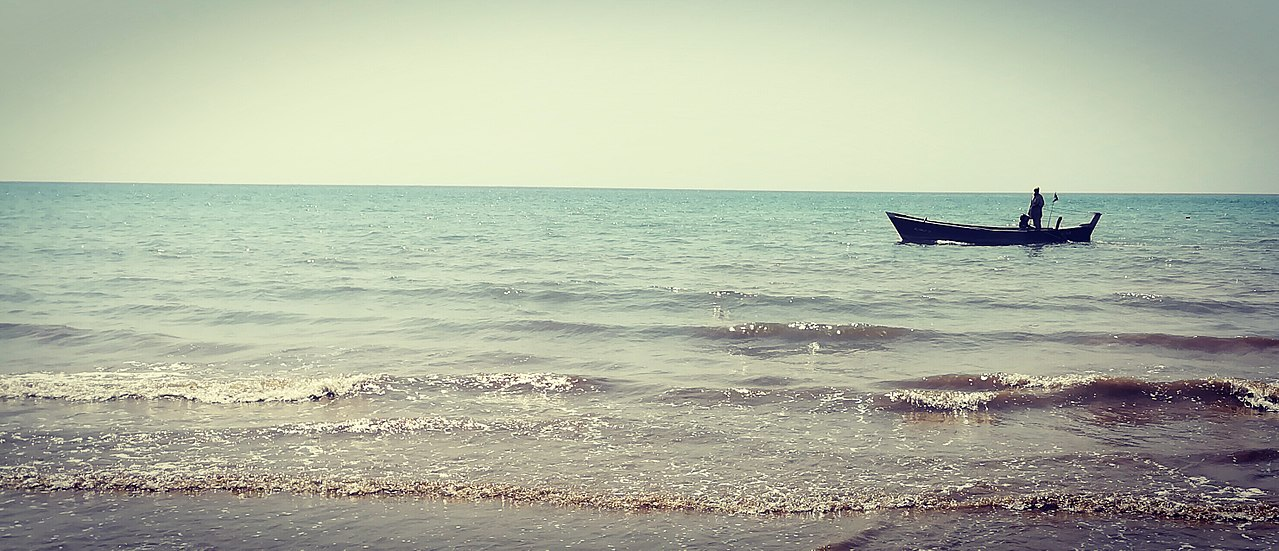
\includegraphics{images/seaside}
	\end{marginfigure}
\end{verbatim}

Offset ca be either a measure or a multiple of \verb|\baselineskip| in 
the format \verb|[*5]|.\todo{improve this part} If you are wondering how 
I inserted this orange bubble, have a look at the \verb|todo| package.

\section{Wide figures and tables}

With the environments \verb|figure*| and \verb|table*| you can insert 
figures which span the whole page width. The caption will be positioned 
below.

Now, if you will excuse me, I will add some more blindtext. \blindtext

\blindtext

\begin{figure*}
	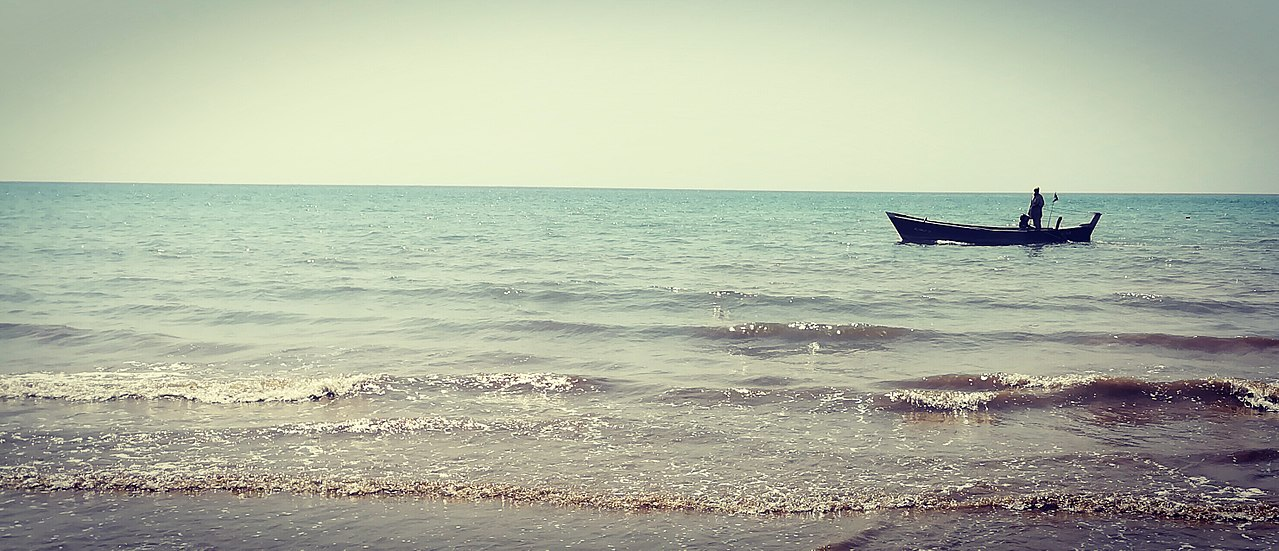
\includegraphics{images/seaside}
	\vspace{-1.2cm}
	\caption[A wide seaside]{A wide seaside, and a wide caption.
		Credits: By Bushra Feroz - Own work, CC BY-SA 4.0, 
		https://commons.wikimedia.org/w/index.php?curid=68724647.
		\blindtext}
\end{figure*}

\section{Image before chapter}

It is relatively easy to insert a figure before the chapter title with 
the help of the \verb|\setchapterpreamble| command. The details are left 
to the reader\sidenote{Check the source code for a hint.}.

Note also that throughout the document I have used different chapter 
title styles, both to experiment and to show some possibilities. 
Customising this is quite easy as well.

\newglossaryentry{computer}
{
  name=computer,
  description={is a programmable machine that receives input,
               stores and manipulates data, and provides
               output in a useful format}
}
\newacronym[longplural={Frames per Second}]{fpsLabel}{FPS}{Frame per Second}

\renewcommand*{\chapterformat}
{
  \enskip\mbox{\scalebox{4}{\thechapter\autodot}}
}
\renewcommand\chapterlinesformat[3]
{
  \parbox[b]{\textwidth}{\hrulefill#2}\par%
  #3%\par\bigskip
  \parbox[b]{\textwidth+\marginparsep+\marginparwidth}{\hrulefill}%
  %\hrule
}
\setchapterpreamble[u]{\margintoc}
\chapter{References}

\section{Citations}

To cite someone \sidecite{Visscher2008,James2013} is very simple: just 
use the \verb|\sidecite| command. It does not have an offset argument 
yet, but it probably will in the future. This command supports multiple 
entries, as you can see, and by default it prints the reference on the 
margin as well as adding it to the bibliography at the end of the 
document. For this setup I used biblatex but I think that workarounds 
are possible \sidecite{James2013}. Note that the citations have nothing 
to do with the text, they are completely random as they only serve the 
purpose to illustrate the feature.

\section{Glossaries and Indices}

I previously defined some glossary entries and now I am going to use 
them, for instance, like this: \gls{computer}. Since we are here, let us 
reference an acronym: this is the full version, \acrfull{fpsLabel}, and 
this is the short one \acrshort{fpsLabel}. These entries will appear in 
the glossary in the backmatter.


%\widepage
%\setpartpreamble{
  %\begin{center}
  %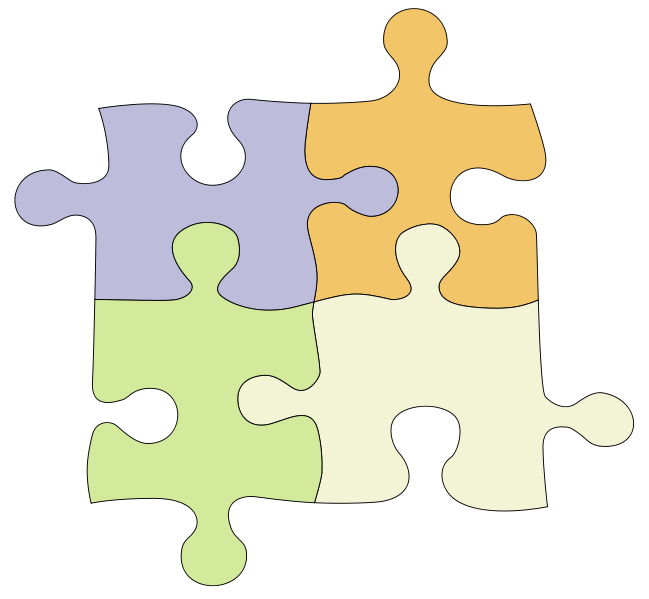
\includegraphics[width=0.8\linewidth]{images/partpre}
  %\captionof{figure}{\url{https://commons.wikimedia.org/wiki/File:Puzzle-4.svg}}
  %\end{center}
%}
%\part{Style}
%\marginpage

%\chapter{TODO}

\appendix

\blinddocument


\backmatter

% Bibliograhy
%\setbibpreamble{References in citation order\par\bigskip}
\printbibliography[heading=bibintoc,title=Bibliography]

% Index
\printindex

% Glossary
%\printglossary[type=\acronymtype, title=Acronyms, toctitle=Acronyms]
\printglossary[title=Special Terms, toctitle=List of terms]

% Back cover
\clearpage
\thispagestyle{empty}
\null%
\clearpage
%\includepdf{pages/cover-back.pdf}

\end{document}
